\chapter{Numerical experiments}
\label{cha:experiments}

The previous chapter showed how much faster the GPU implementation is compared to the same algorithm implemented on the CPU. This significant increase in performance allows for new numerical experiments.

In this chapter we will present results from a number of experiments performed to explore the numerical precision of the implementation and to validate the results against prior research. The simulation parameters used in the experiments can be found in the Appendix~\ref{app:parameters}.

We begin by looking at tumbling orbits, a very delicate experiment requiring good numerical precision. Next we reproduce a very interesting physical phenomenon of letting a spherical cloud of fibers sediment and validate our results against similar experiment by others. Furthermore, we will have a brief exploration of the effects of the number of fibers and the concentration of fibers on the spherical cloud simulation. All experiments are run with the new GPU algorithm  implemented in the thesis. The linear system is solved using the direct solver from MAGMA in order to avoid variations in the run time.

\section{Tumbling orbits}
\label{sec:example_ring}

To verify that the single precision GPU implementation is able to replicate the result using the original double precision code, we perform a very simple experiment where a small number of fibers are set up with perfectly symmetrical positions and orientations. Initially, all fibers are evenly distributed on a circle and aligned vertically with gravity. During the simulation, while sedimenting, the fibers begin to rotate from their vertical orientation towards a horizontal position. Afterwards, they continue rotating back into the vertical position. This motion is referred to as a tumbling motion and as long as there are no disturbances or numerical precision issues it repeats forever.

This simple but very interesting problem has also been simulated by Gustavsson and Tornberg,~\cite{Gustavsson2009}. Additionally an even more simplified version with only two fibers was studied both numerically and experimentally by Jung et al.,~\cite{Jung2006}. This example is thus ideally suited to test and verify the numerical precision of the GPU implementation. A visualization of the result using the GPU code for $16$ fibers evenly distributed around a circle with a radius of $0.55$, is shown in Fig.~\ref{fig:ring_simulation}.

\begin{figure}[!htbp]
  \centering
  \begin{subfigure}[h]{0.45\textwidth}
    \centering
    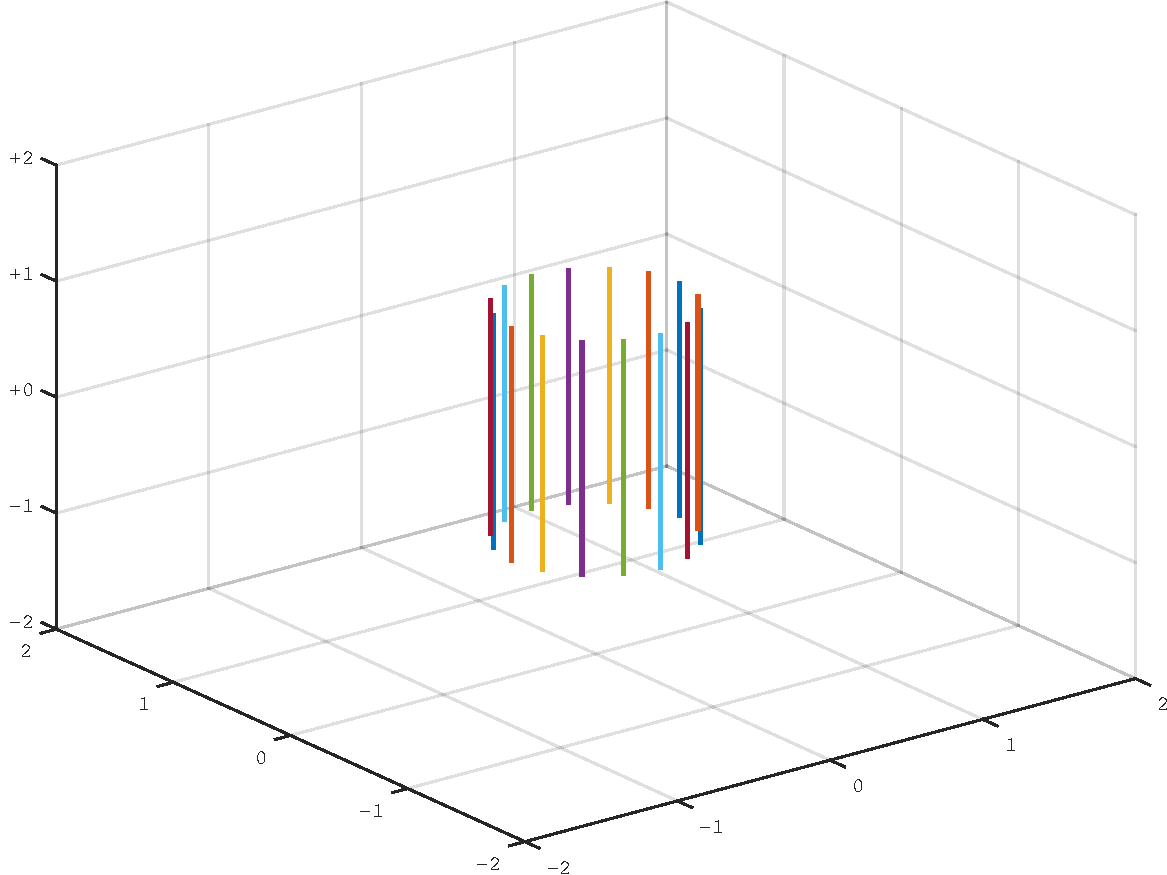
\includegraphics[width=\textwidth]{img/ring_00000.pdf}
    \caption{$t=0$}\label{fig:ring_simulation_1a}
  \end{subfigure}
  \begin{subfigure}[h]{0.45\textwidth}
    \centering
    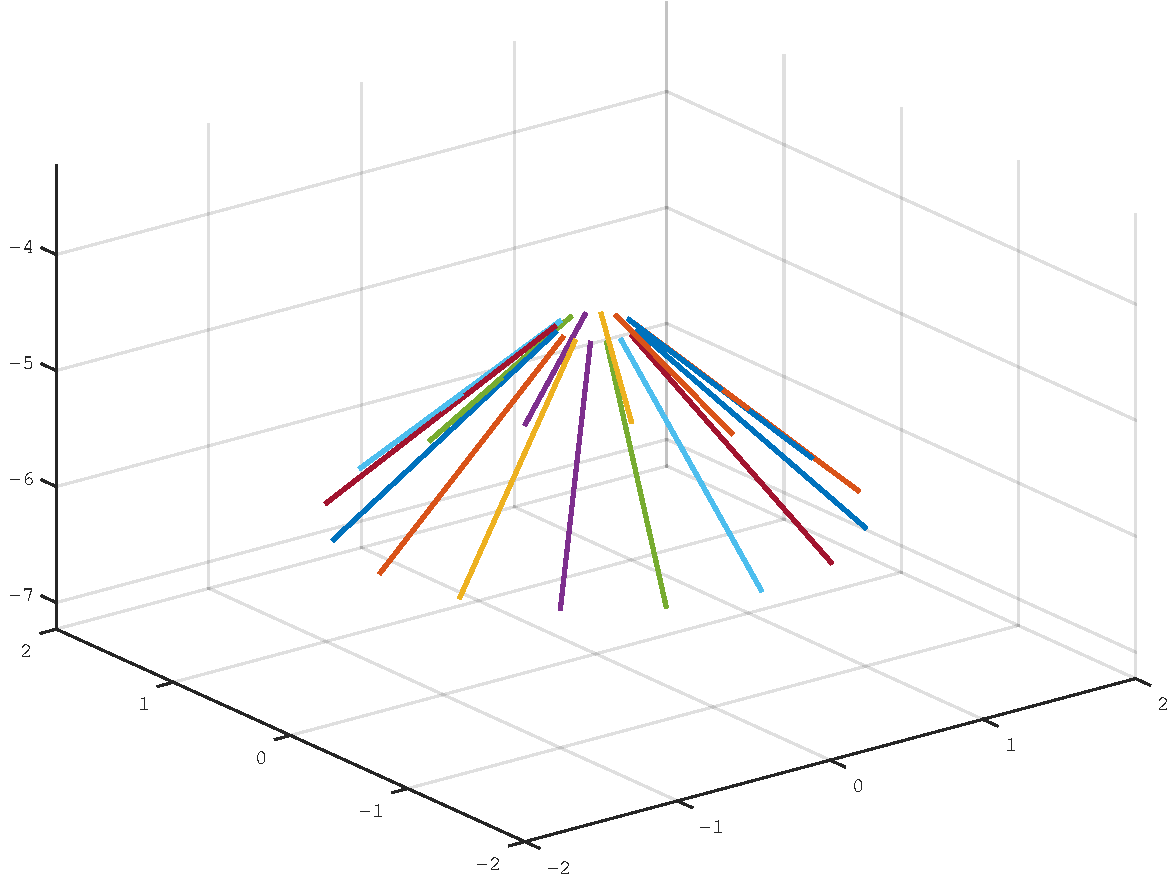
\includegraphics[width=\textwidth]{img/ring_00015.pdf}
    \caption{$t=15$}\label{fig:ring_simulation_1b}
  \end{subfigure}
  \begin{subfigure}[h]{0.45\textwidth}
    \centering
    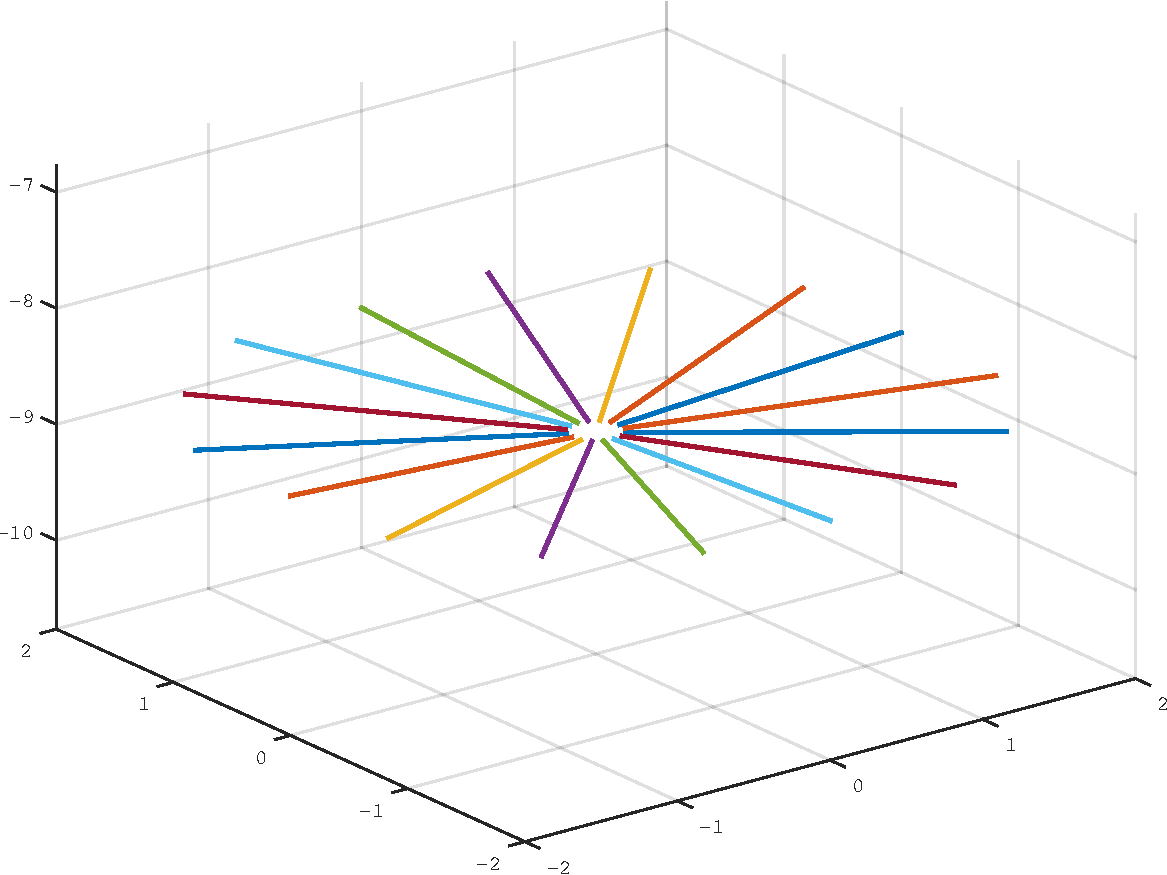
\includegraphics[width=\textwidth]{img/ring_00030.pdf}
    \caption{$t=30$}\label{fig:ring_simulation_1c}
  \end{subfigure}
  \begin{subfigure}[h]{0.45\textwidth}
    \centering
    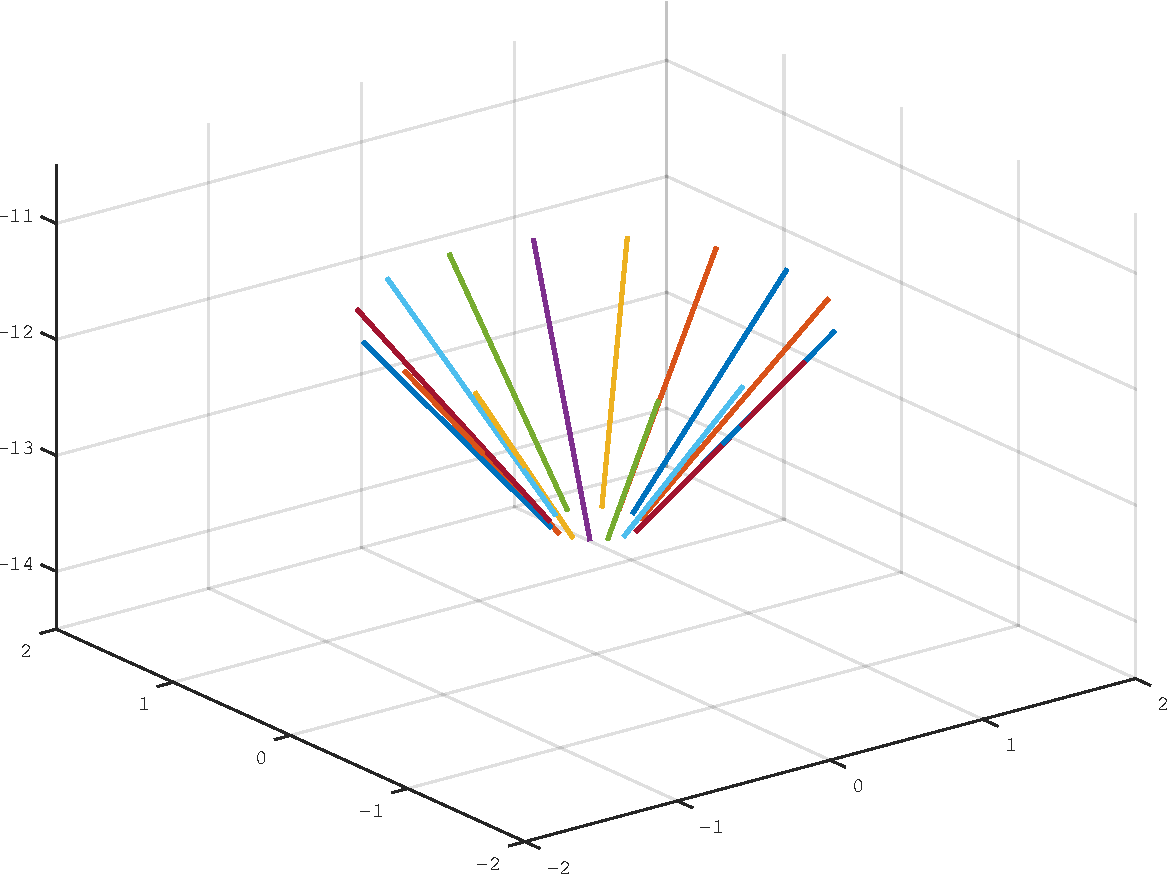
\includegraphics[width=\textwidth]{img/ring_00045.pdf}
    \caption{$t=45$}\label{fig:ring_simulation_1d}
  \end{subfigure}
  \caption[Visualization of tumbling orbits.]{Visualization of tumbling orbits. Small number of perfectly symmetrically distributed fibers around a circle are allowed to sediment due to gravity. The fibers perform a periodical motion alternating between a vertical and horizontal orientation in the direction to gravity.}
  \label{fig:ring_simulation}
\end{figure}

Initially, the fibers are aligned vertically and are sedimenting with the maximum velocity. As they rotate into the horizontal orientation the velocity decreases and reaches its minimum once the fibers are perpendicular to the direction of gravity. Afterwards on their way back to vertical orientation the velocity increases again.

Fig.~\ref{fig:ring_sedimentation_velocity} shows a graph of the sedimentation velocity of a single fiber over time for both the single precision GPU code and the original double precision Fortran code. As the same force acts on all fibers and they perform the same motion they all have the same sedimentation velocity. For this particular setup the maximum velocity is ${\sim}3.8$ and the minimum velocity is ${\sim}2.2$. The graphs clearly shows the periodical rotation the fiber perform. This result perfectly captures the expected result obtained from prior simulation and experiments. The difference in velocity between the two implementations is of the order $10^{-4}$. Hence, even for this delicate experiment, where a small disturbance will cause a deviation from the periodic orbit, the single precision accuracy is sufficient.

\begin{figure}[!htbp]
  \centering
  \begin{tikzpicture}
    \begin{axis}[
      xlabel={Timestep},
      ylabel={Velocity},
      height={207pt},
      unbounded coords=discard,
      xmin=0,xmax=200,
      ymin=-4,ymax=-2,
      ]

      \addplot[color=set12, very thick] table[x=Timestep,y=Single] {charts/ring_sedimentation.csv};
      \addplot[color=set11, loosely dashed, ultra thick] table[x=Timestep,y=Double] {charts/ring_sedimentation.csv};
    \end{axis}
  \end{tikzpicture}
  \caption[Comparison of sedimentation velocity for single- and double-precision simulation.]{Comparison of sedimentation velocity for single precision (solid line) and double precision (dashed line) simulation.}
  \label{fig:ring_sedimentation_velocity}
\end{figure}

\section{Sedimenting of a spherical cloud}
\label{sec:example_sphere}

The next example is a more chaotic system with a large number of interacting fibers. In the numerical experiment $2000$ fibers are initially distributed in the form of a spherical cloud. Both their positions and orientations are random inside the cloud. Due to gravity the cloud will sediment. This experiment has been studied in several papers, e.g.~\cite{Bulow2015}\cite{Metzger2007}\cite{Park2010}. It is especially interesting because the observed results only occur if enough fibers are simulated. Our GPU simulation is able to efficiently handle up to $2000$ fibers and is thus ideally suited for studying this example.

\begin{figure}[!htbp]
  \centering
  \begin{subfigure}[h]{0.4\textwidth}
    \centering
    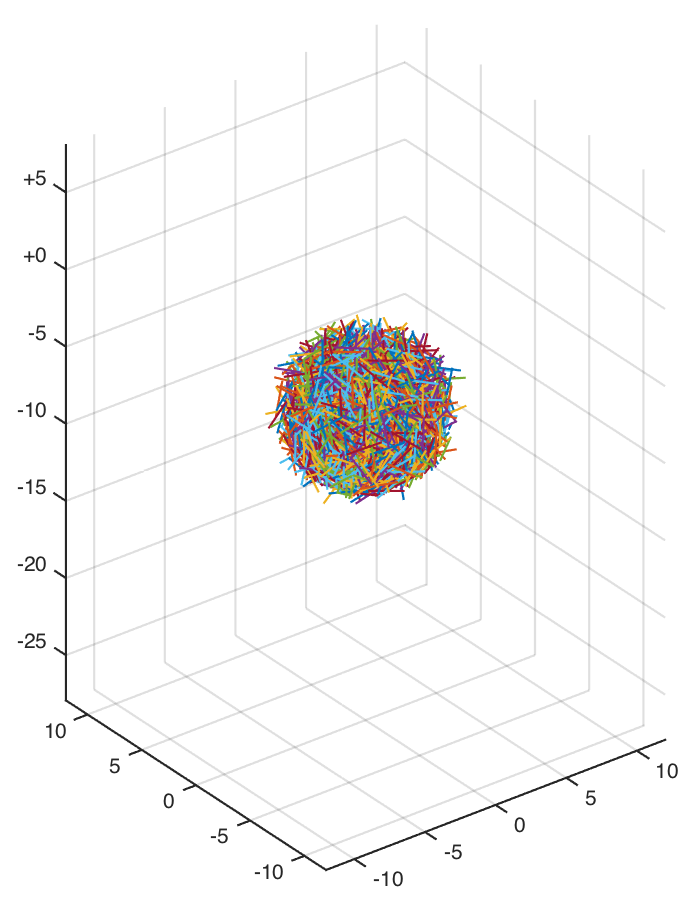
\includegraphics[width=\textwidth]{img/state_00000.pdf}
    \caption{$t=0$}\label{fig:sphere_simulation_1a}
  \end{subfigure}
  \begin{subfigure}[h]{0.4\textwidth}
    \centering
    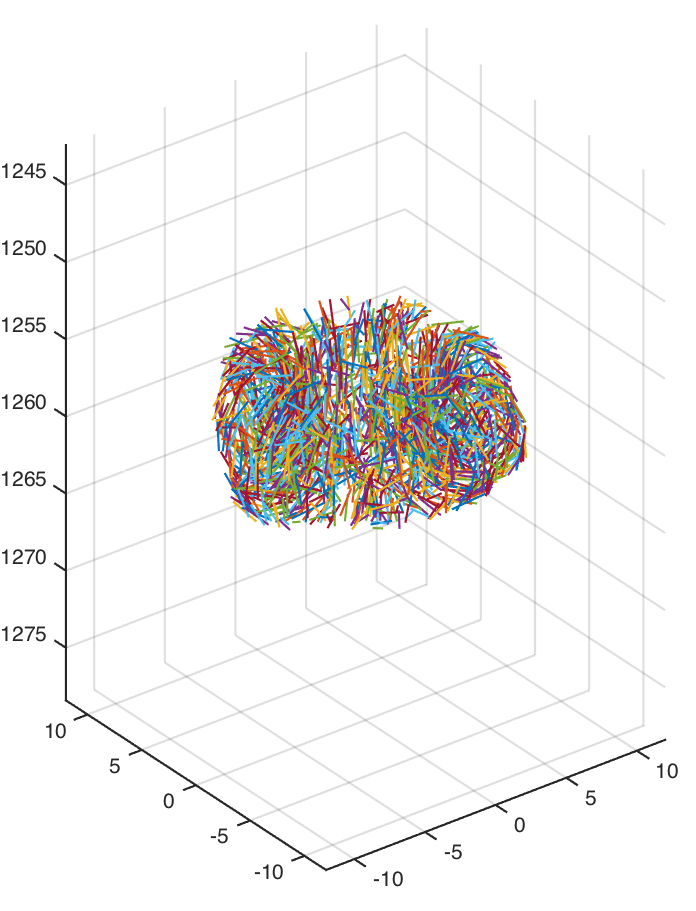
\includegraphics[width=\textwidth]{img/state_00250.pdf}
    \caption{$t=300$}\label{fig:sphere_simulation_1b}
  \end{subfigure}
  \begin{subfigure}[h]{0.4\textwidth}
    \centering
    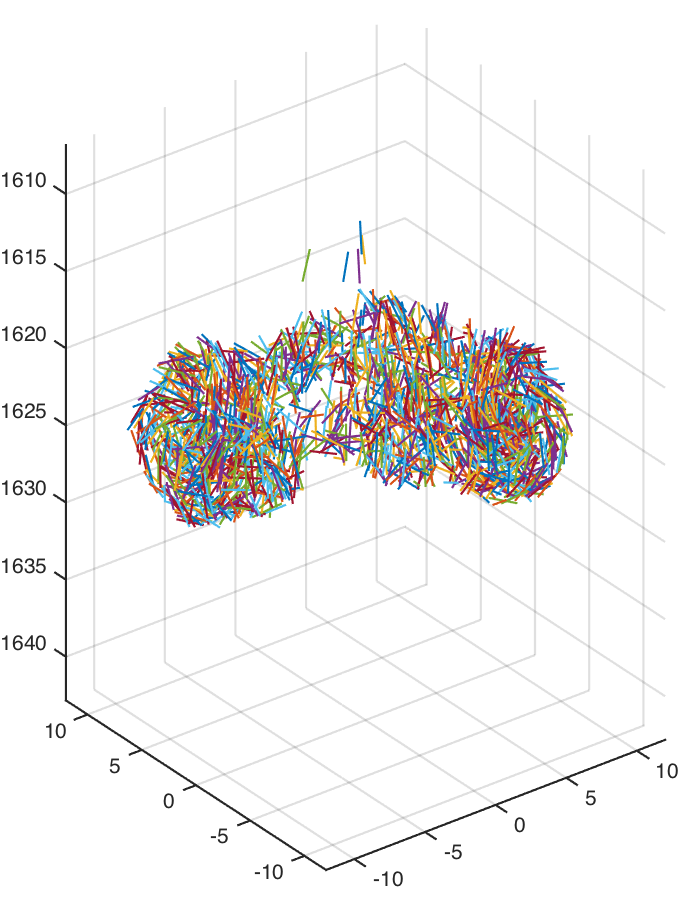
\includegraphics[width=\textwidth]{img/state_00350.pdf}
    \caption{$t=350$}\label{fig:sphere_simulation_1c}
  \end{subfigure}
  \begin{subfigure}[h]{0.4\textwidth}
    \centering
    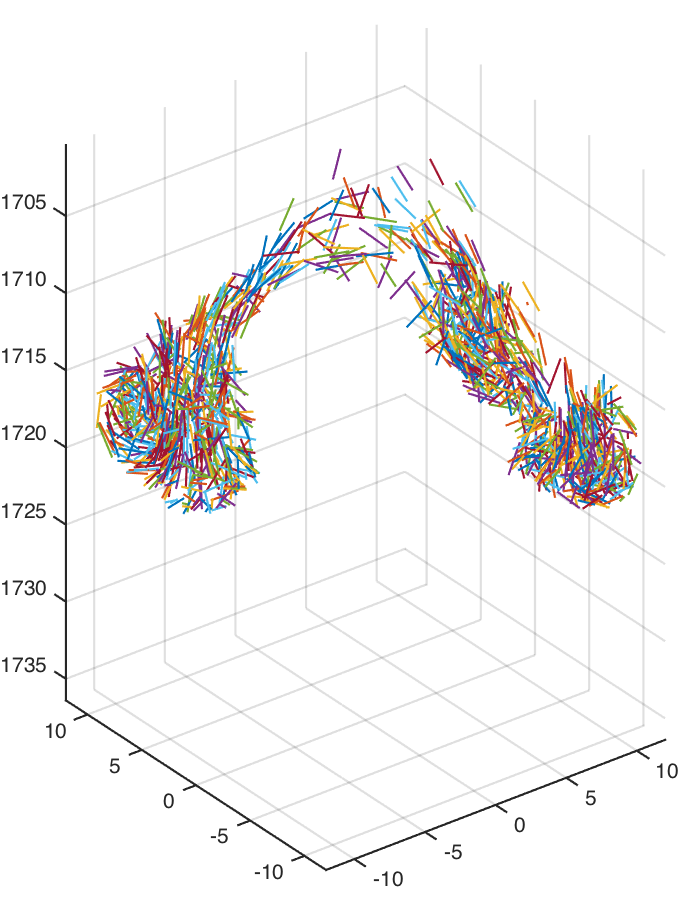
\includegraphics[width=\textwidth]{img/state_00380.pdf}
    \caption{$t=380$}\label{fig:sphere_simulation_1d}
  \end{subfigure}
  \caption[Visualization of sedimenting spherical cloud.]{Visualization of sedimenting spherical cloud. Fibers are randomly distributed in the form of a spherical cloud and sediment due to gravity. The fibers proceed to form a turning torus. Eventually the torus breaks up into subclusters.}
  \label{fig:sphere_simulation}
\end{figure}

In Fig.~\ref{fig:sphere_simulation} we can see how the interacting fibers, beginning from the spherical shape, slowly start to form a continuously turning torus. Even though the behavior is more chaotic due to the large number of fibers and the random initial setup, this turning torus somewhat resembles the result for the tumbling orbits in Sec.~\ref{sec:example_ring}.

After some time the torus breaks and the fibers are split into multiple smaller cloudlets, which continue to sediment separately and slowly form their own smaller torus. However, due to tiny variations these toruses can be harder to see. 

The simulation of the presented example only takes ${\sim}8$ seconds per timestep using the GPU implementation. Consequently it is possible to perform the $500$ time steps of the simulation in a little bit over $1$ hour. Simulating this many fibers in such a short time will allow for new research of this interesting phenomenon. One interesting question is to determine what influences the stability of the torus that is, when time does the torus break up.

\subsection{Spherical cloud break-up}
\label{subsec:sphere_break}
To begin investigating this question we first define the stability of the torus in terms of the break up time. How to determine the exact break up time of the torus is quite challenging. This problem was also examined by Park et al.,~\cite{Park2010}. In~\cite{Park2010} the break-up time is defined as the moment when the torus starts to bend prior to actually breaking. Unfortunately, they do not define a metric that determines the exact break up time. Based on the work in~\cite{Park2010} we have developed a new measure of the break-up time.

We use the same definition for the torus as described by Park et al.,~\cite{Park2010}. First we compute the initial horizontal radius $R_0$ of the sphere. As the cloud sediments and starts forming the torus, there is a small leakage fibers in its vertical tail. To find these fibers, such that they can be excluded from the active set of fibers defining the torus, we exclude all fibers with a distance larger than $R_0$ in the direction of gravity from the center of mass of the torus. For the remaining fibers we can compute the horizontal radii $R_x$ and $R_y$ by computing the distance from the center of the torus and the mean sedimentation velocity $V_z$. The torus shape is illustrated in Fig~\ref{fig:torus_shape} and the metrics over time for a sample run with $2000$ fibers and an average distance of $0.4$ in Fig.~\ref{fig:torus}. The horizontal radii $R_x$ and $R_y$ of the torus and the percentage of fibers remaining in the torus are shown in Fig.~\ref{fig:torus_radius} and Fig.~\ref{fig:torus_fibers}. The curves show the expected loss of fibers and the increasing torus radius.

\begin{figure}[!htbp]
  \centering
  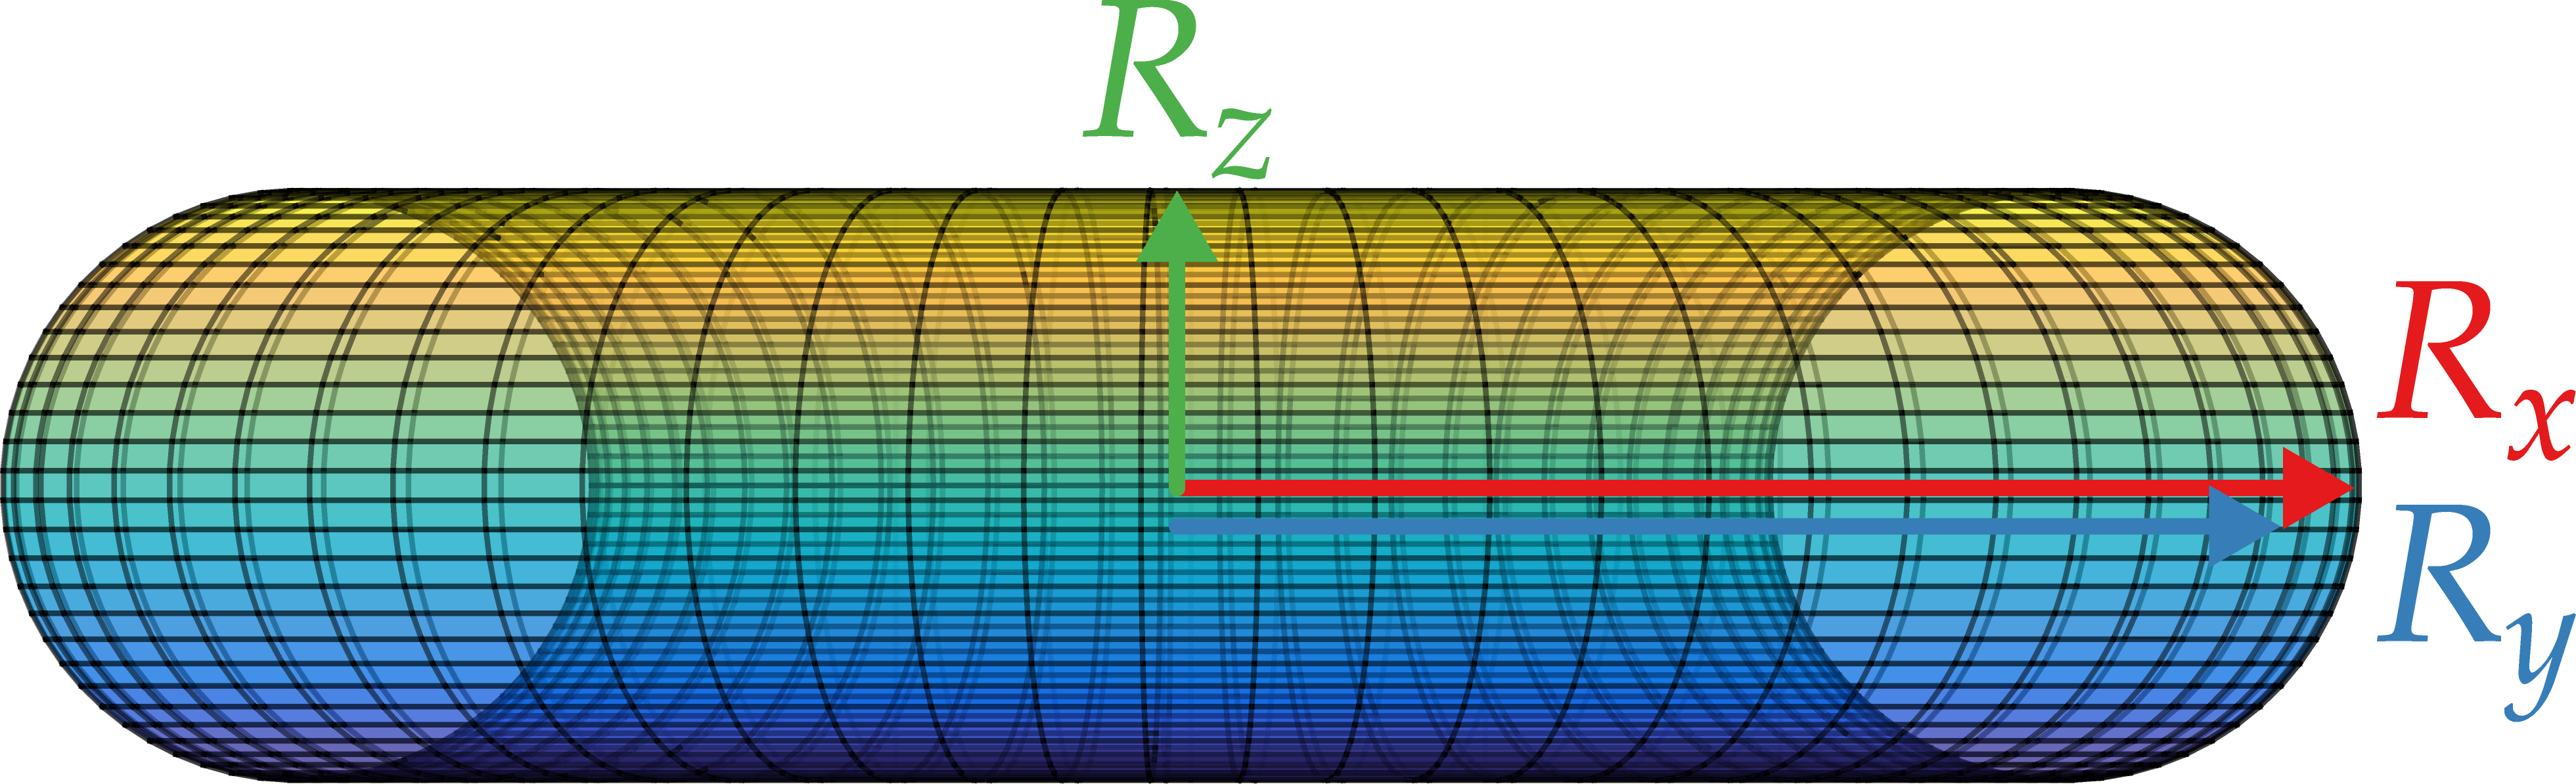
\includegraphics[width=0.6\textwidth]{img/torus3.png}
  \caption[Torus Shape.]{Torus Shape. The torus is defined by the two horizontal radii $R_x$ and $R_y$ and the vertical radius in the direction of gravity $R_z$.}
  \label{fig:torus_shape}
\end{figure}

\begin{figure}[!htbp]
  \centering
  \begin{subfigure}[h]{.48\textwidth}
	  \begin{tikzpicture}
	    \begin{axis}[
	      xlabel={Timestep},
	      ylabel={Radius},
	      width={\textwidth},
	      unbounded coords=discard,
	      xmin=0,xmax=500,
	      ymin=5,ymax=20,
	      grid=major,
	      every axis label/.append style={font=\sffamily\footnotesize},
	      ]
	
	      \addplot[color=set11, very thick] table[x=Timestep,y=RadiusX,col sep=comma] {charts/sphere_2000_0040.csv};
	      \addplot[color=set12, densely dotted, very thick] table[x=Timestep,y=RadiusY,col sep=comma] {charts/sphere_2000_0040.csv};
	
		\legend{$R_x$,$R_y$}
	    \end{axis}
	  \end{tikzpicture}
    \caption{Torus horizontal radius.}\label{fig:torus_radius}
  \end{subfigure}
  \begin{subfigure}[h]{.48\textwidth}
	  \begin{tikzpicture}
	    \begin{axis}[
	      xlabel={Timestep},
	      ylabel={Fibers in torus (\%)},
	      width={\textwidth},
	      unbounded coords=discard,
	      xmin=0,xmax=500,
	      ymin=0.9,ymax=1.0,
	      grid=major,
	      legend pos=north east,
	      every axis label/.append style={font=\sffamily\footnotesize},
	      ]
	
	      \addplot[color=set11, very thick] table[x=Timestep,y=NormalizedN,col sep=comma] {charts/sphere_2000_0040.csv};
	
	    \end{axis}
	  \end{tikzpicture}
    \caption{Percentage of remaining fibers.}\label{fig:torus_fibers}
  \end{subfigure}
  \begin{subfigure}[h]{.48\textwidth}
	  \begin{tikzpicture}
	    \begin{axis}[
	      xlabel={Timestep},
	      ylabel={Radius},
	      width={\textwidth},
	      unbounded coords=discard,
	      xmin=0,xmax=500,
	      ymin=1,ymax=2.5,
	      grid=major,
	      every axis label/.append style={font=\sffamily\footnotesize},
	      ]
	
	      \addplot[color=set12, mark=*,mark options={fill=white}, very thick] table[x=Timestep,y=RadiusZStd,col sep=comma] {charts/sphere_2000_0040_highlight.csv}
	node[pos=444, pin={[pin edge={color=set12, very thick}]min}]{};
	      \addplot[color=set11, very thick] table[x=Timestep,y=RadiusZStd,col sep=comma] {charts/sphere_2000_0040.csv};
	    \end{axis}
	  \end{tikzpicture}
    \caption{Torus $\text{Radius}_z$ Standard Deviation.}\label{fig:torus_deviation}
  \end{subfigure}
  \begin{subfigure}[h]{.48\textwidth}
	  \begin{tikzpicture}
	    \begin{axis}[
	      xlabel={Timestep},
	      ylabel={Velocity},
	      width={\textwidth},
	      unbounded coords=discard,
	      xmin=0,xmax=500,
	      ymin=-5,ymax=-2,
	      grid=major,
	      legend pos=north east,
	      every axis label/.append style={font=\sffamily\footnotesize},
	      ]
	
	      \addplot[color=set11, very thick] table[x=Timestep,y=VelocityZ,col sep=comma] {charts/sphere_2000_0040.csv};
	
	    \end{axis}
	  \end{tikzpicture}
    \caption{Mean sedimentation velocity.}\label{fig:torus_velocity}
  \end{subfigure}
  \caption[Time evolution of the sedimenting torus.]{Time evolution of the sedimenting torus. In the beginning the torus loses some fibers and the horizontal radii $R_x$ and $R_y$ increase slowly. The vertical radius $R_z$ undergoes a periodical contraction and expansion, which can also be seen in the peridocal change in the sedimentation velocity $V_z$. The eventual moment of the break-up of the torus is defined as the minimum standard deviation of the vertical radius $R_z^{\text{std}}$.}
  \label{fig:torus}
\end{figure}

In Fig.~\ref{fig:torus_deviation} we present the standard deviation of the radius in the direction of gravity as a function of time. We observe that the standard deviation of the radius in the direction of gravity for all fibers in the torus continuously decreases until it reaches a minimum value after which it starts to increase again. The time when the standard deviation reaches the minimum value can be identified visually to a few moments before the torus breaks up. We verified this metric manually against many simulations and it showed a great agreement with the visual moment of break-up. Using this metric we are now able to investigate the effect of the number and concentration of fibers on the stability and break up time of the torus.

A surprising result was that the standard deviation of the radius in the direction of gravity, $R_z$, seems to oscillate with time, see Fig.~\ref{fig:torus_deviation}. This implies that the torus is periodically expanding and shrinking until it breaks up. The same behavior can also be seen in the mean sedimentation velocity, $V_z$, of the torus, Fig.~\ref{fig:torus_velocity}. This periodical change in velocity is similar to the motion observed in the simple tumbling orbits experiment presented in Sec.~\ref{sec:example_ring}. Hence, it seems like the turning torus with $2000$ fibers is a more chaotic version of the simplified tumbling orbits.

\subsection{Fiber concentration effect on break-up time}
\label{subsec:effect_concentration}

The first parameter to explore is the concentration of fibers, which we measure in terms of the average distance between a fiber and its closest neighbor. In the numerical experiments, we fixed the number of fibers at $2000$ and varied the concentration in the spherical cloud by varying its initial radius. The break-up time is estimated using the metric defined in Sec.~\ref{subsec:sphere_break}.

In Fig.~\ref{fig:concentration_breakup} the break-up time is presented as a function of the average distance between the fibers. We can see that there is a clear correlation. When the average distance between the fibers increases, i.e. a decrease in concentration, the time until the torus breaks up increases. When the cloud sediments and starts forming a torus, a large rotating velocity field is created in the fluid. The strength of this field depends on how strong the interaction between the fibers is. When the fibers are far apart the interaction between the fibers is small and the rotating motion will not be as strong, leading to a longer break-up time.

\begin{figure}[!htbp]
  \centering
  \begin{tikzpicture}
    \begin{axis}[
      xlabel={Concentration},
      ylabel={Break-up time step},
      width={0.618033989\textwidth},
      unbounded coords=discard,
      ymin=0,ymax=1500,
      xmin=0,xmax=14,
      grid=major,
      ]

      \addplot[color=set11, mark=*,mark options={fill=white}, very thick] table[x=Concentration,y=Break,col sep=comma] {charts/concentration_breakup.csv};

    \end{axis}
  \end{tikzpicture}
  \caption[Effect of fiber concentration on torus break up time.]{Effect of fiber concentration on torus break up time. The concentration of fibers is defined in terms of the average distance between fibers in the spherical cloud.}
  \label{fig:concentration_breakup}
\end{figure}

\subsection{Number of fibers effect on break-up time}
\label{subsec:effect_number}

The second parameter we studied was the number of fibers. In this set of experiments, the concentration is fixed by keeping the average distance between the fibers fixed to $0.4$. We measure the break up time as we vary the number of fibers from $100$ to $2000$. In Fig.~\ref{fig:number_breakup} the result is displayed. Here we find that there is a positive correlation between the number of fibers and the break-up time, however not as strong as in the case when we varied the concentration in Sec.~\ref{subsec:effect_concentration}. These results match the results found by Park et al.,~\cite{Park2010}.

The results presented in Sec.~\ref{subsec:effect_concentration} and Sec.~\ref{subsec:effect_number} show that both fiber concentration and the number of fibers affect the break-up time of the torus. Future research should explore these correlations closer and include other studies such as the dependence of the initial shape of the cloud on the process.

\begin{figure}[!htbp]
  \centering
  \begin{tikzpicture}
    \begin{axis}[
      xlabel={Number of fibers},
      ylabel={Break-up time step},
      width={0.618033989\textwidth},
      unbounded coords=discard,
      xmin=0,xmax=2000,
      ymin=0,ymax=1500,
      grid=major,
      ]
      \addplot[color=set11, mark=*,mark options={fill=white}, very thick] table[x=M,y=Break] {charts/number_breakup.csv};

    \end{axis}
  \end{tikzpicture}
  \caption[Effect of number of fibers on torus break up time.]{Effect of number of fibers on torus break up time. Here the concentration of fibers is constant.}
  \label{fig:number_breakup}
\end{figure}

These two results show that both the concentration and the number of fibers have an effect on the break up time of the torus. Future research should explore these correlations closer as our tests only looked at two parameters in isolation. How other parameters, like external forces, the numerical accuracy and the initial fiber distribution affect the stability of the torus are promising questions.

\section{Cloud of fibers with different densities}
\label{sec:mixed_density_sphere}

The final experiment resembles a setup investigated by Bülow et al.,~\cite{Bulow2015}, where the authors studied the settling behavior of a spherical cloud with particles of different size. Here, we will study the sedimentation of a spherical cloud with fibers of different densities. We divide the total number of fibers into two different density groups and arrange them inside a spherical cloud, which sediments due to gravity. To separate the two groups visually, they are colored in red and blue. The blue group has the lower density and the red group the higher density. The ratio between the densities is set to $\text{blue} / \text{red}= 0.75 / 1.0$.

Fig.~\ref{fig:unmixed_sphere} shows the results from a simulation at different timesteps, where the two density groups are initially separated into the top and bottom half of the spherical cloud. Since the fibers are clearly separated, this particular configuration is referred to as an unmixed cloud. Initially the fibers with the higher density are in the upper half of the cloud and the fibers with the lower density are in the bottom half, see Fig.~\ref{fig:mixing_top_a}. After a short time, we can see in Fig.~\ref{fig:mixing_top_b} that the high density fibers have almost completely dropped through the low density fibers, leaving a large trail of low density fibers behind. After a while, the high and low density fibers are almost totally separated and proceed independently of each other to form the characteristic torus, see Fig.~\ref{fig:mixing_top_c}. As the torus formed by the high density fibers grows in size and becomes less dense its sedimentation velocity will decrease. As depicted in Fig.~\ref{fig:mixing_top_d} the low density group of fibers will eventually catch up with the high density fibers and drop through the larger torus. The tori are not very stable and soon afterward they will break up.

\begin{figure}[!htbp]
  \centering
  \begin{subfigure}[h]{0.24\textwidth}
    \centering
    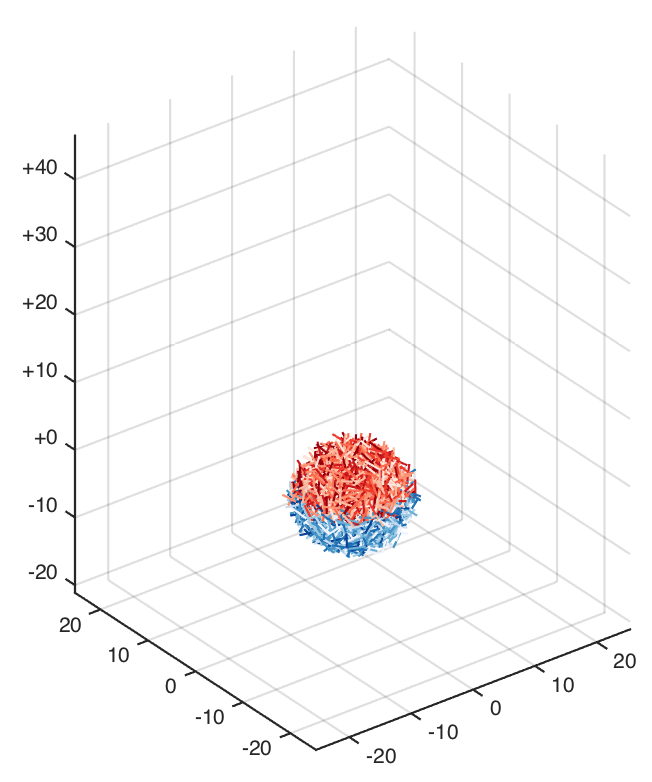
\includegraphics[width=\textwidth]{img/mixing/top_00000.pdf}
    \caption{$t=0$}\label{fig:mixing_top_a}
  \end{subfigure}
  \begin{subfigure}[h]{0.24\textwidth}
    \centering
    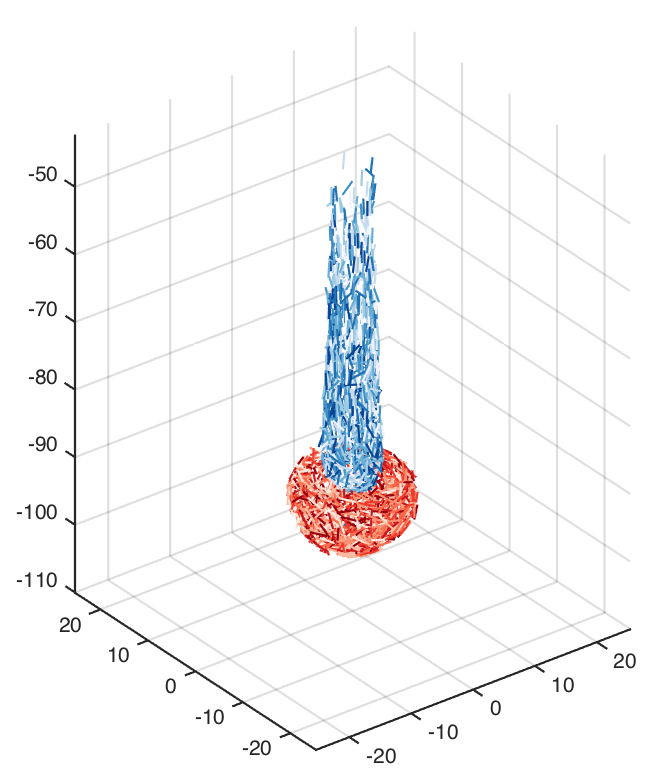
\includegraphics[width=\textwidth]{img/mixing/top_00020.pdf}
    \caption{$t=20$}\label{fig:mixing_top_b}
  \end{subfigure}
  \begin{subfigure}[h]{0.24\textwidth}
    \centering
    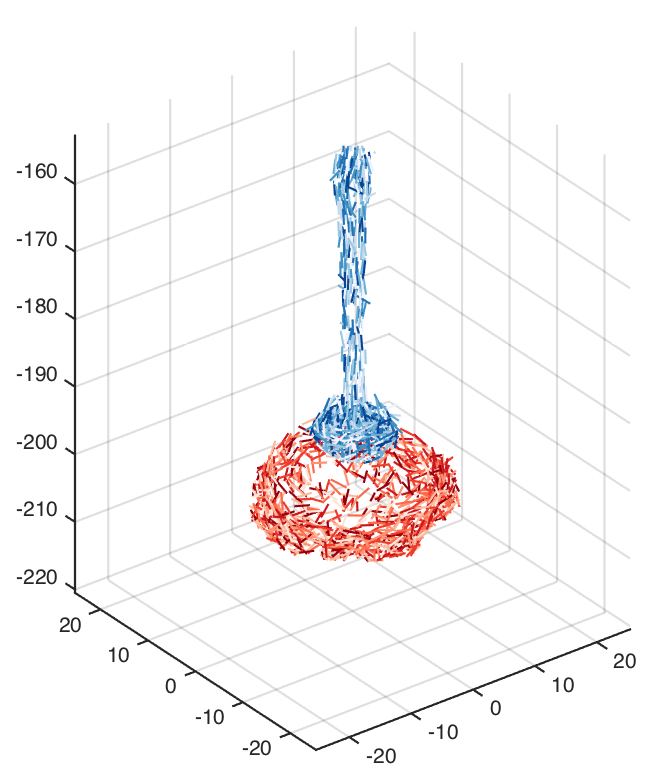
\includegraphics[width=\textwidth]{img/mixing/top_00060.pdf}
    \caption{$t=60$}\label{fig:mixing_top_c}
  \end{subfigure}
  \begin{subfigure}[h]{0.24\textwidth}
    \centering
    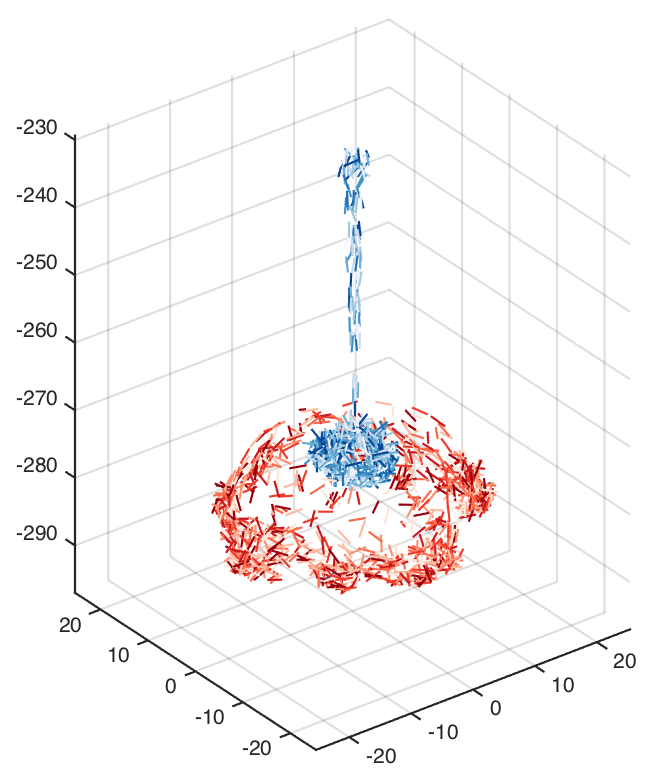
\includegraphics[width=\textwidth]{img/mixing/top_00100.pdf}
    \caption{$t=100$}\label{fig:mixing_top_d}
  \end{subfigure}
  \caption[Unmixed cloud.]{Unmixed cloud. Initially the high density fibers (red) are in the top half of the cloud and the low density fibers (blue) are in the bottom half.}
  \label{fig:unmixed_sphere}
\end{figure}

Next we perform a similar experiment but with the fibers of different densities randomly distributed inside the cloud, see Fig.~\ref{fig:mixing_random_a}. We refer to this setup as a mixed cloud. The beginning of the simulation behaves similar to the unmixed case, but the separation does not happen as fast and far fewer low density fibers are lost in the tail of the cloud, Fig.~\ref{fig:mixing_random_b}. Once again two tori are formed, but in contrast to the unmixed case, both groups of fibers stay closer together, which prevents the fibers of different densities from completely separating. In Fig.~\ref{fig:mixing_random_c} we can see how the high density torus is sucked down by the passing low density torus. During the following timesteps the two tori appear to form an interlocked torus, which continues to sediment, Fig.~\ref{fig:mixing_random_d}. Eventually the interlocked torus breaks up and fibers scatter. 

\begin{figure}[!htbp]
  \centering
  \begin{subfigure}[h]{0.24\textwidth}
    \centering
    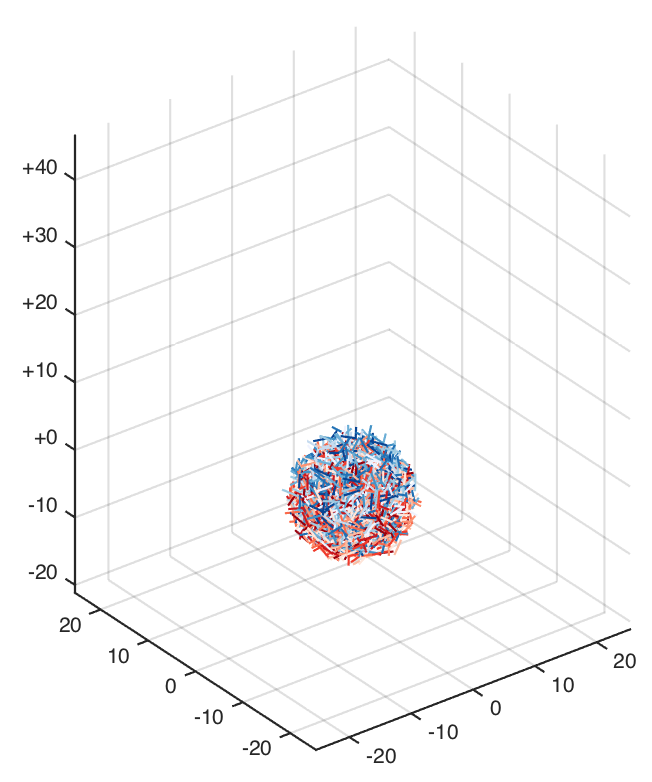
\includegraphics[width=\textwidth]{img/mixing/random_00000.pdf}
    \caption{$t=0$}\label{fig:mixing_random_a}
  \end{subfigure}
  \begin{subfigure}[h]{0.24\textwidth}
    \centering
    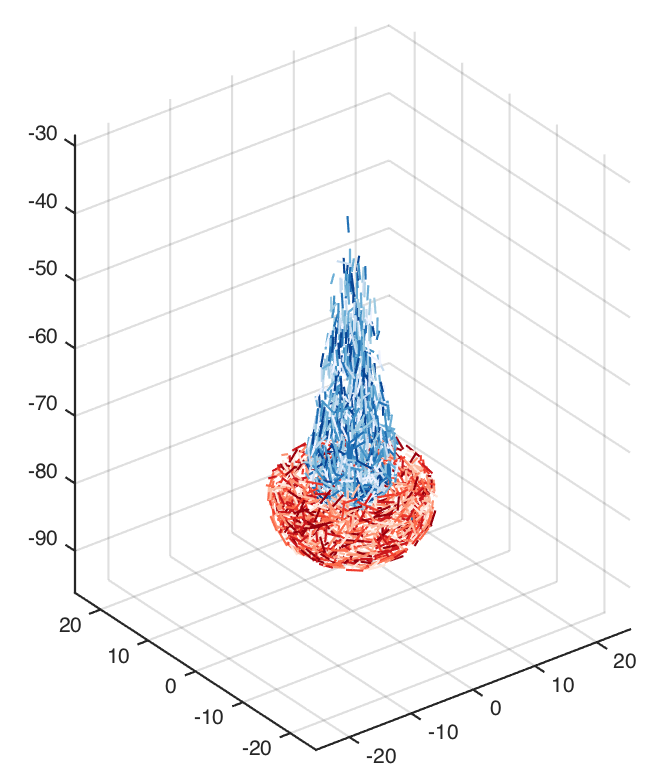
\includegraphics[width=\textwidth]{img/mixing/random_00020.pdf}
    \caption{$t=20$}\label{fig:mixing_random_b}
  \end{subfigure}
  \begin{subfigure}[h]{0.24\textwidth}
    \centering
    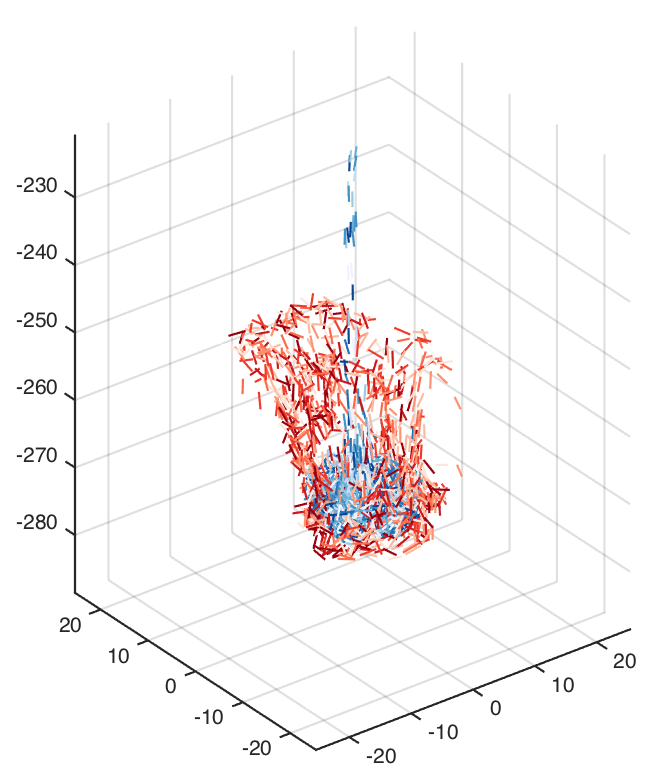
\includegraphics[width=\textwidth]{img/mixing/random_00100.pdf}
    \caption{$t=100$}\label{fig:mixing_random_c}
  \end{subfigure}
  \begin{subfigure}[h]{0.24\textwidth}
    \centering
    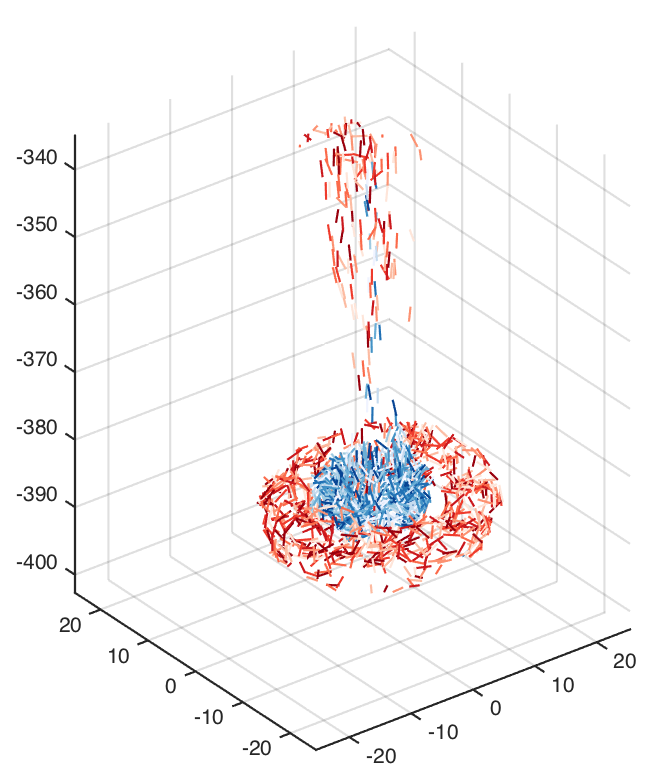
\includegraphics[width=\textwidth]{img/mixing/random_00150.pdf}
    \caption{$t=150$}\label{fig:mixing_random_d}
  \end{subfigure}
  \caption[Mixed cloud.]{Mixed cloud. Initially the high (red) and low (blue) density fibers are randomly mixed inside the cloud.}
  \label{fig:mixed_sphere}
\end{figure}

The results displayed for the mixed and unmixed cloud with rigid fibers do agree on a qualitative level with the results presented in Bülow et al.,~\cite{Bulow2015}. However, both simulation methods and setups are very different which makes a quantitive comparison very challenging. Furthermore our experiment are only in an initial stage and many more experiments have to be carried out to get a deeper understanding of the behavior of rigid fibers of different densities in a spherical cloud. Exploring the impact of initial fiber configuration, the density ratio and the fiber concentration are all exciting future research opportunities.
